\chapter{Static Schedule}
\label{chap:Static}
This chapter largely follows the results of \citet{Pegden}. The aim is to derive a method for choosing an optimal static schedule. A static schedule is a sequence of $n$ customer arrival times $t_{1}, \ldots, t_{n}$ chosen at the start of service and fixed for the duration of service. 

For simplicity, these results assume the customer service times are independent and identically distributed (iid) exponential random variables with mean $\mu$. There is a single server. All customers are punctual and arrive at their scheduled arrival time.

\section{Objective Function}
The optimal schedule minimises the expected cost, which is a linear combination of the expected total customers' waiting time and total expected server availability time.

Denote the expected waiting time of customer $i$ as $w_{i}$. The expected total customers' waiting time is the sum of the individual customer's expected waiting times.
\begin{equation}
	\mathbb{E} \Big[\text{total customer's waiting time} \Big] = \sum_{i = 1}^{n} w_{i}
\end{equation}

Instead of solving for the customer arrival times, it is easier to solve for the arrival time of the first customer $t_{1}$ and the customer interarrival times $\mathbf{x} = (x_{1}, \ldots, x_{n - 1})$ where $x_{i} = t_{i + 1} - t_{i}$. The expected total server availability time is the expected time from the start of service until the end of service. This the sum of the last customer's scheduled arrival time, the last customer's expected waiting time and the last customer's expected service time.
\begin{equation}
	\mathbb{E} \Big[\text{total server availability time} \Big] = \left( t_{1} + \sum_{i = 1}^{n - 1} x_{i} \right) + w_{n} + \mu
\end{equation}

Denote $c_{W}$ and $c_{I}$ as the per unit time cost of the expected total customer's waiting time and the per unit time cost of the expected total server availability time respectively. The objective function to be minimised is thus,
\begin{equation}
	\phi (t_{1}, \mathbf{x}) = c_{W} \sum_{i = 1}^{n} w_{i} + c_{S} \left[ t_{1} + \sum_{i = 1}^{n - 1} x_{i} + w_{n} + \mu \right]
\end{equation}

The first customer should obviously be scheduled for the start of service so $t_{1} = 0$. Moreover, can scale the objective function by dividing by $(c_{W} + c_{S})$ and defining $\gamma = \frac{c_{S}}{c_{W} + c_{S}}$.
\begin{equation}
	\phi (\mathbf{x}) = (1 - \gamma) \sum_{i = 1}^{n} w_{i} + \gamma \left[ \sum_{i = 1}^{n - 1} x_{i} + w_{n} + \mu \right]
	\label{eqn:StaticObjective}
\end{equation}

The optimal static schedule is thus the interarrival times that minimise Equation~\ref{eqn:StaticObjective}

\section{Expected Waiting Time}
We want to express $w_{i}$ (i.e., the expected waiting time of customer $i$) as a function of the interarrival times $\mathbf{x}$. If there are $j$ customers in the system just prior to the arrival of customer $i$, then $w_{i} = j \mu$ by the memoryless property of the exponential distribution. The number of customers in the system refers to both customers being served and customers waiting for service.

Denote the number of customers in the system just prior to the arrival of customer $i$ as $N_{i}$. Thus, the expected waiting time of customer $i$ is given by
\begin{equation}
	w_{i} = \sum_{j = 0}^{i - 1} (j \mu) \mathbb{P} (N_{i} = j)
	\label{eqn:StaticWaiting}
\end{equation}

The probability of a given number of customers in the system can be expressed recursively. This probability depends on the number of departures from the system between the arrival of customer $(i - 1)$ and customer $i$. The number of departures is the minimum of $(N_{i - 1} + 1)$ and a Poisson random variable with mean $\frac{x_{i - 1}}{\mu}$.

The full recursive expression for the probability of $j$ customers in the system immediately before the arrival of customer $i$ is
\begin{equation}
	\mathbb{P} (N_{i} = j) = \begin{cases} 1 & \text{for $i = 1$, $j = 0$} \\
	\sum_{k = 1}^{i - 1} \mathbb{P} (N_{i - 1} = k - 1) \left[ 1 - \sum_{l = 0}^{k - 1} \frac{x_{i - 1}^{l}}{\mu^{l} l!} \mathrm{e}^{\frac{- x_{i - 1}}{\mu}}\right] & \text{for $i \geq 2$, $j = 0$} \\
	\sum_{k = 0}^{i - j - 1} \mathbb{P} (N_{i - 1} = j + k - 1) \left[ \frac{x_{i - 1}^{k}}{\mu^{k} k!} \mathrm{e}^{\frac{- x_{i - 1}}{\mu}} \right] & \text{for $i \geq 2$, $j \geq 1$} \end{cases}
	\label{eqn:StaticProbSystem}
\end{equation}

\section{Computing the Objective Function}
\citet{Pegden} suggest a similar algorithm to Algorithm~\ref{alg:StaticObjective} for computing the value of the objective function given by Equation~\ref{eqn:StaticObjective} for a given vector $\mathbf{x}$ and parameters $\gamma$ and $\mu$.
\begin{algorithm}[htb]
\caption{Return $\phi (\mathbf{x})$ for a given vector $\mathbf{x}$, $\gamma$ and $\mu$}
\begin{algorithmic}
\Function{ObjectiveFunction}{$\mathbf{x}$,$\gamma$,$\mu$}
    \For {$i = 1, 2, \ldots, n$}
    	\For {$j = 0, 1, \ldots, (i - 1)$}
    		\State compute $\mathbb{P} (N_{i} = j)$ by Equation~\ref{eqn:StaticProbSystem}
    	\EndFor
    \EndFor
    \For {$i = 1, 2, \ldots, n$}
    	\State compute $w_{i}$ by Equation~\ref{eqn:StaticWaiting}
    \EndFor
    \State \Return $\phi (\mathbf{x})$ computed by Equation~\ref{eqn:StaticObjective}
\EndFunction
\end{algorithmic}
\label{alg:StaticObjective}
\end{algorithm}

\section{Example Models}
\subsection{Model for Two Customers}
\label{sec:StaticTwoCust}
We consider the simplest case of this model where there are two customers to be scheduled (i.e., $n = 2$). As the first customer is scheduled to arrive at the start of service, the only unknown variable is the optimal interarrival time between the first and second customer (i.e., $x_{1}$).

By Equation~\ref{eqn:StaticWaiting}, the expected waiting times of the two customers are
\begin{align}
	w_{1} & = 0 \\
	w_{2} & = \mu \mathrm{e}^{\frac{- x_{1}}{\mu}}
\end{align}

By Equation~\ref{eqn:StaticObjective}, the objective function to be minimised is given by
\begin{equation}
	\phi (x_{1}) = \mu \left[ \gamma + \exp \left( \frac{- x_{1}}{\mu} \right) \right] + \gamma x_{1}
\end{equation}

This objective function is convex as
\begin{equation}
	\forall x_{1} \ \ \phi'' (x_{1}) = \frac{1}{\mu} \exp \left( \frac{- x_{1}}{\mu} \right) > 0
\end{equation}

Due to the convexity of the objective function, the optimal policy that minmises $\phi (x_{1})$ can be found by solving:
\begin{equation}
	\phi' (x_{1}) = 0 \implies - \exp \left( \frac{- x_{1}}{\mu} \right) + \gamma = 0
\end{equation}

Therefore, the optimal policy is:
\begin{equation}
	x_{1}^{*} = \argmin_{x_{1}} \phi (x_{1}) = - \mu \ln \gamma
\end{equation}

As the server availability cost increases relative to the customer waiting cost (i.e., $\gamma$ increases), the second customer is scheduled to arrive earlier (i.e., $x_{1}^{*}$ decreases).

Unfortunately, as \citet{Pegden} found, no general algebraic solution exists for more than two customers (i.e., $n \geq 3$). All other cases need to be solve numerically. \citet{Pegden} proved that the objective function $\phi (\mathbf{x})$ is convex for $n = 1, 2, 3, 4$. Moreover, they conjecture that it appears to be convex for general $n$, but are unable to prove it.

\subsection{Model for 15 Customers}
The more interesting case concerns scheduling a larger number of customers. We consider here the case of $n = 15$. Without loss of generality, can let $\mu = 1$. For $\mu \neq 1$, the solutions found are the optimal values of $\mu \mathbf{x} = (\mu x_{1}, \ldots, \mu x_{n - 1})$.

Minimising the objective function is a constrained optimization problem. A numeric solution can be found using $\texttt{scipy.optimize.minimize}$ in Python.

\begin{figure}[htb]
	\centering
	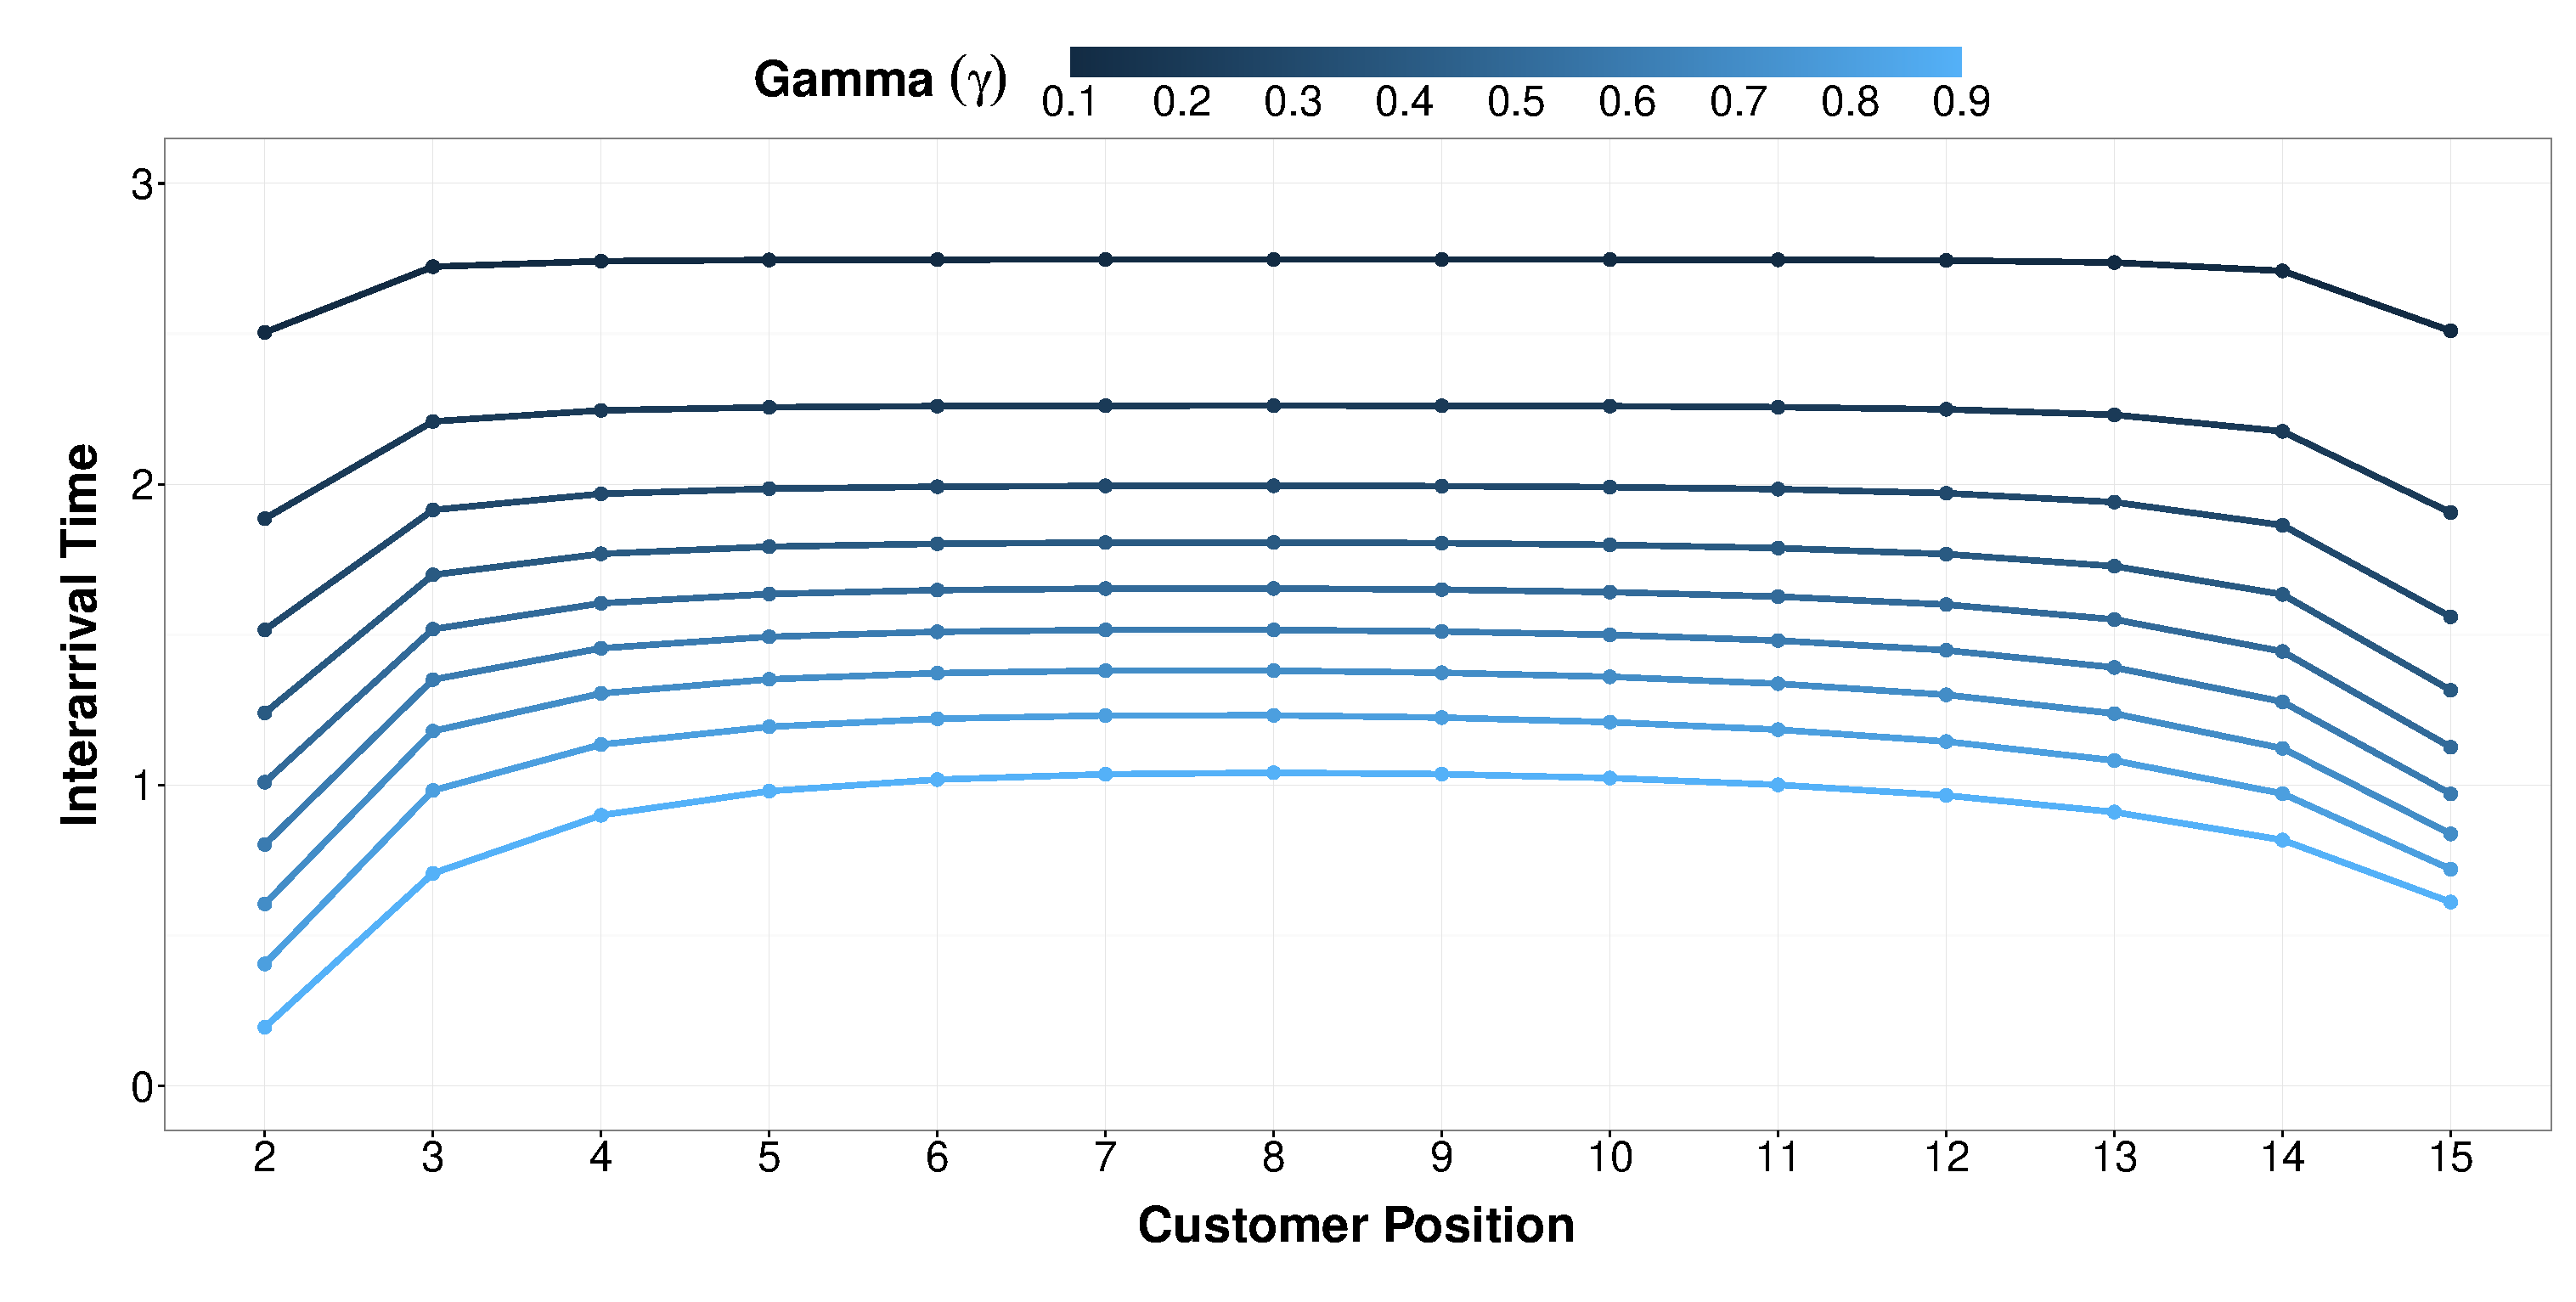
\includegraphics[width = 0.85\textwidth]{Static_Line_Interarrival_Gamma.eps}
	\caption{}
\end{figure}

\begin{figure}[htb]
	\centering
	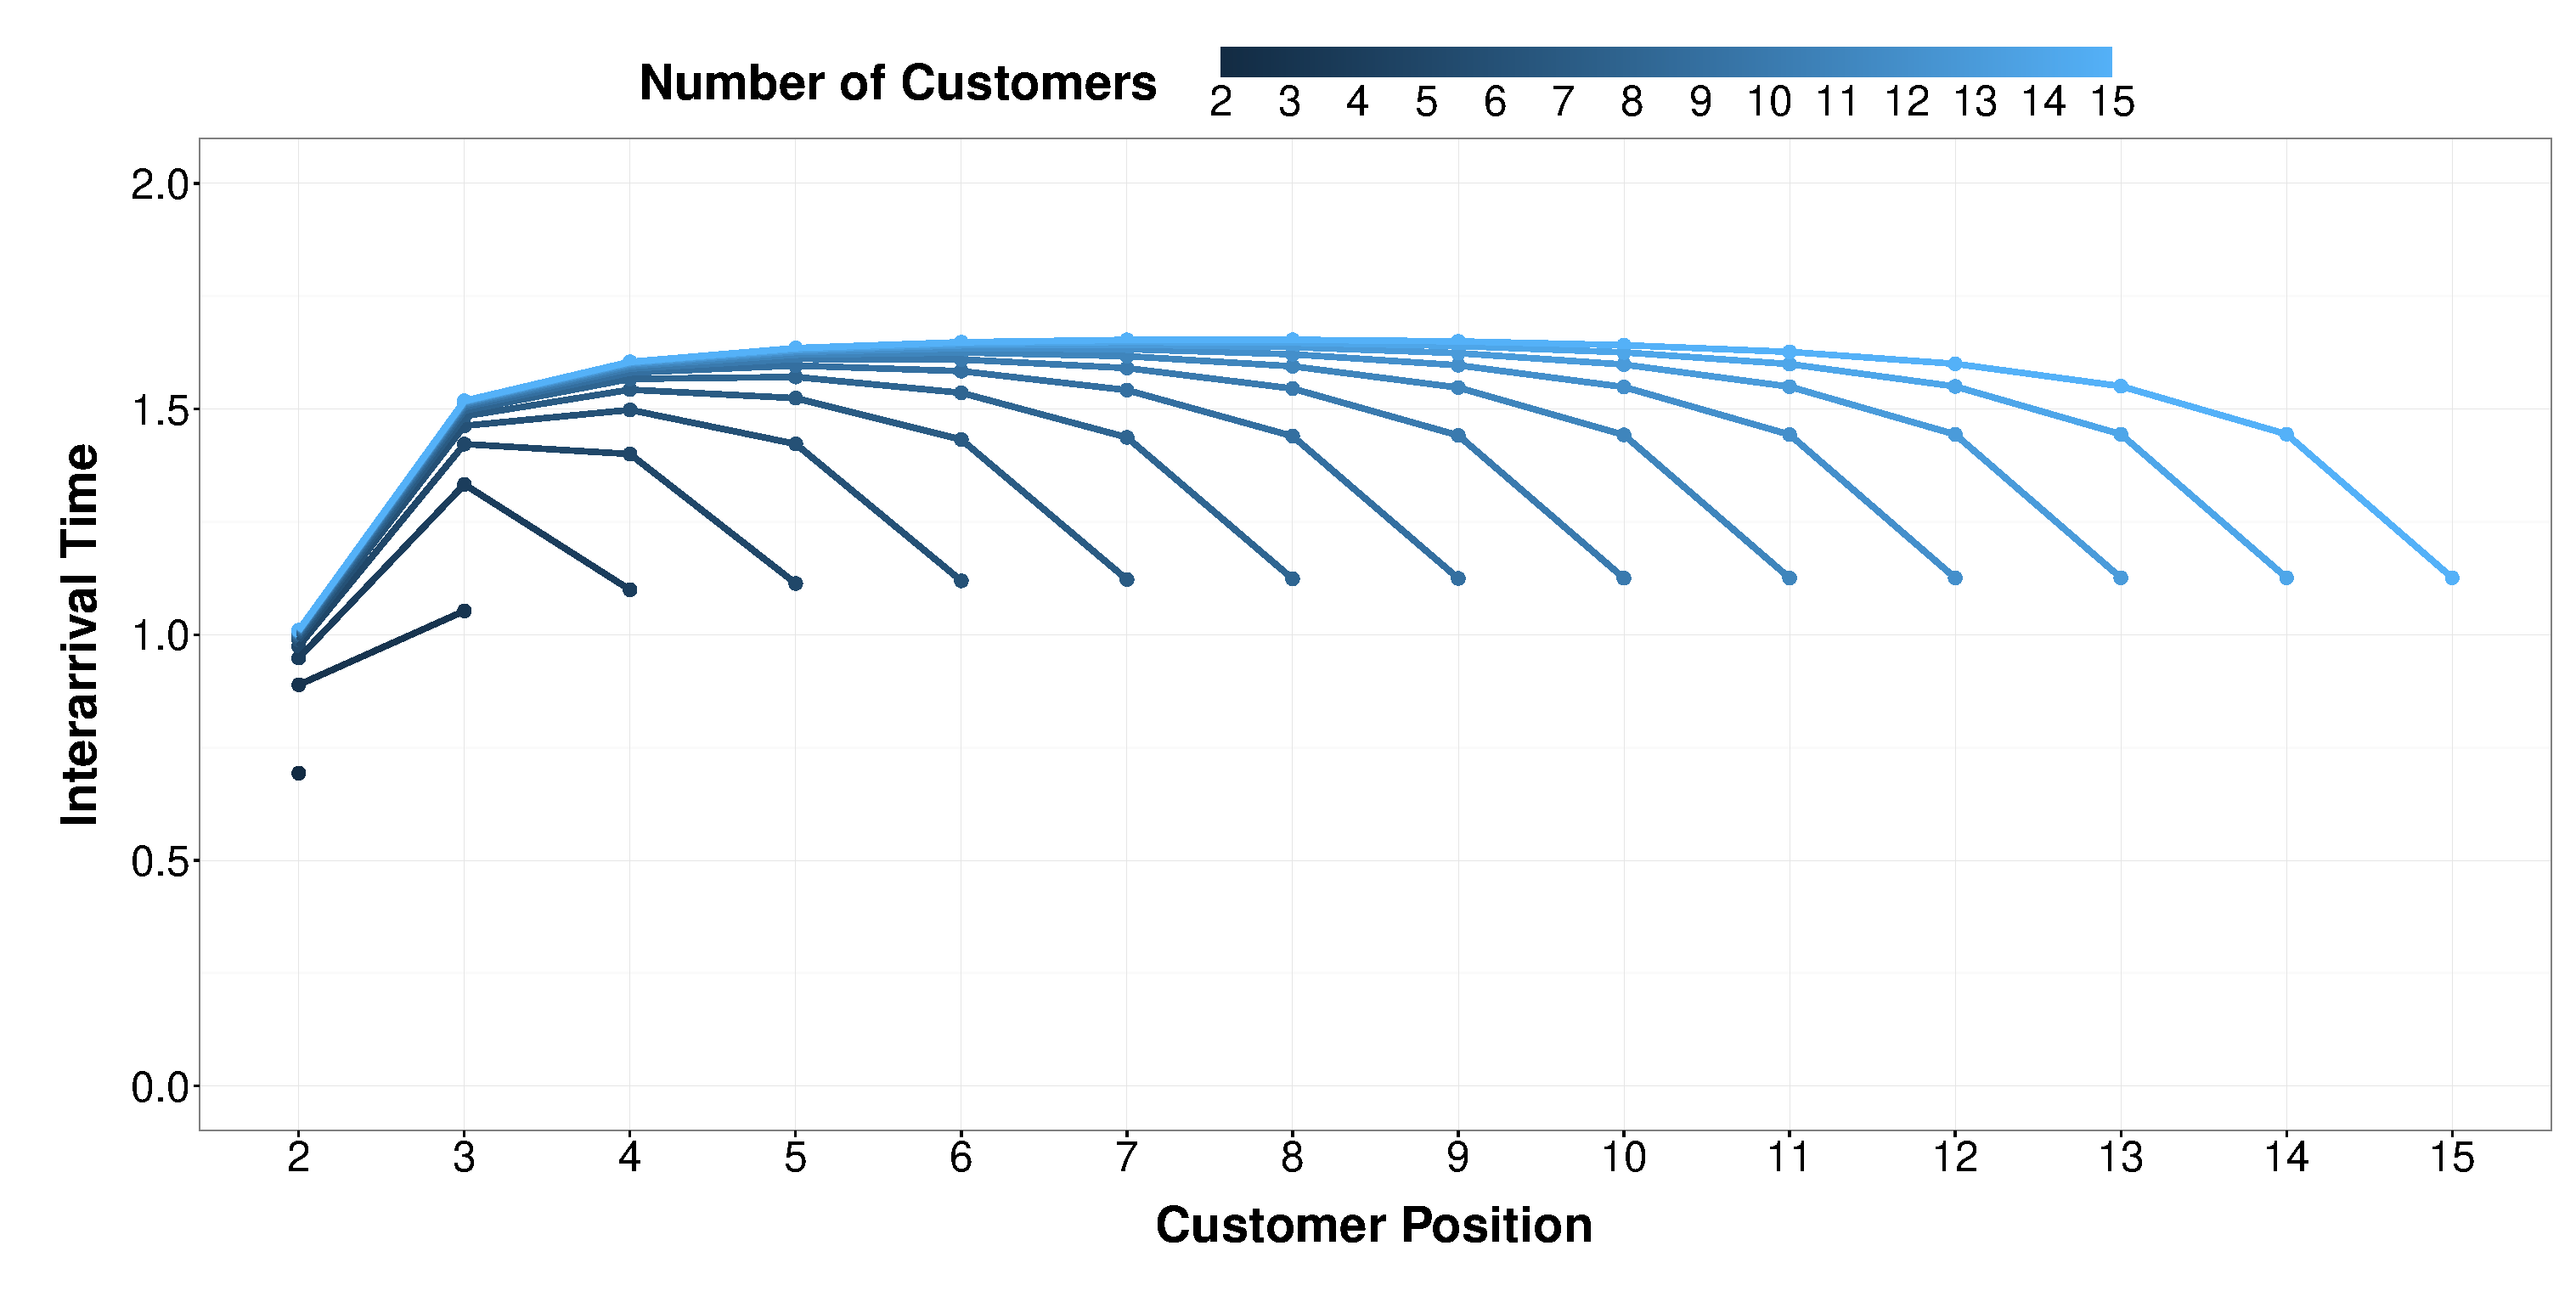
\includegraphics[width = 0.85\textwidth]{Static_Line_Interarrival_Num.eps}
	\caption{}
\end{figure}










































